\label{impl_exp}

\subsubsection{RMSD Benchmarks}
\label{sec:RMSD}
RMSD algorithm for the present test case, represents a task for which computational workload per frame is smaller than I/O workload per frame ($t_{compute_{per-frame}}$ = 0.09 ms, $t_{IO_{per-frame}}$ = 0.3 ms, thus $\tcomp/\tIO \approx 0.3$). 
We showed previously that the RMSD task only scaled well up to 24 cores, on a single compute node on \emph{Comet} (and similarly also only on a
single node on other machines), using either dask or MPI \cite{Khoshlessan:2017ab}. 
Although, it is not clear that the root cause is the same for dask and MPI, here we focus on the MPI
implementation (via \package{mpi4py} \cite{Dalcin:2011aa, Dalcin:2005aa}) for its greater simplicity than dask, in order to
better understand the cause for the poor scaling across nodes.

For both dask and MPI we observed stragglers, individual workers or
MPI ranks, that take much longer to complete than mean execution time of all other workers or ranks. 
Waiting for these stragglers destroys strong scaling performance, as shown in Figure \ref{fig:MPIscaling}, \ref{fig:MPIspeedup} for MPI. 

In the example run in Figure \ref{fig:MPIranks}, ten ranks out of 72 take almost 65~s whereas the
remaining ranks only take about 40~s. The detailed breakdown of the time spent on each rank (Figure \ref{fig:MPIranks}) shows that time
for the actual computation, \tcomp, is fairly constant across ranks. 
The time spent on reading data from the shared trajectory file on the Lustre file system into memory, \tIO, shows variability across different ranks. 
Stragglers, however, appear to be defined by occasional much larger \emph{communication} times, \tcomm (lines 25-30 in \ref{alg:RMSD}), that are on the order of 30~s in this example. 
For other ranks, \tcomm varies across different ranks and for a few ranks $\tcomm < 10$~s or is barely measurable. 
This initial analysis (especially Figure \ref{fig:MPIranks}) indicates that communication is a major issue. 

\begin{figure}
\centering
\begin{subfigure}{.4\textwidth}
  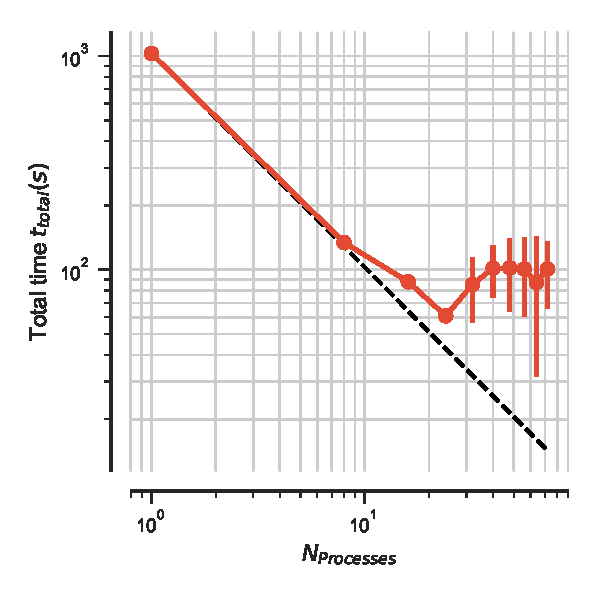
\includegraphics[width=\linewidth]{figures/main-RMSD-t_total.pdf}
  \caption{Scaling total}
  \label{fig:MPIscaling}
\end{subfigure}
\hfill
\begin{subfigure}{.4\textwidth}
  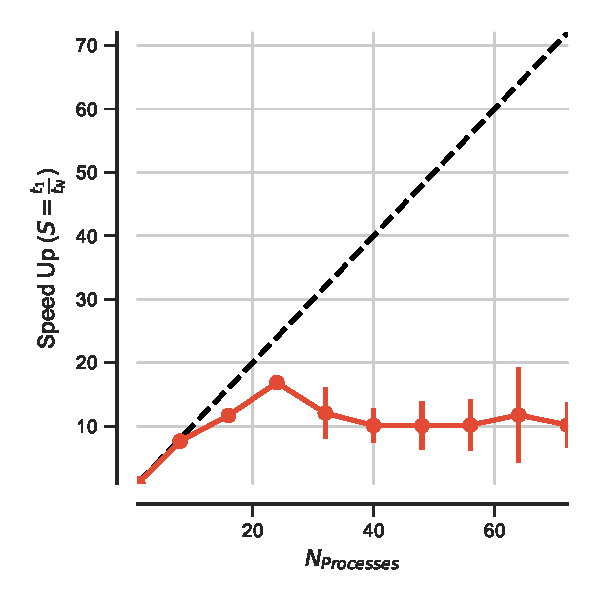
\includegraphics[width=\linewidth]{figures/main-RMSD-speed_up.pdf}
  \caption{Speed-up}
  \label{fig:MPIspeedup}
\end{subfigure}
\bigskip

\begin{subfigure} {.8\textwidth}
  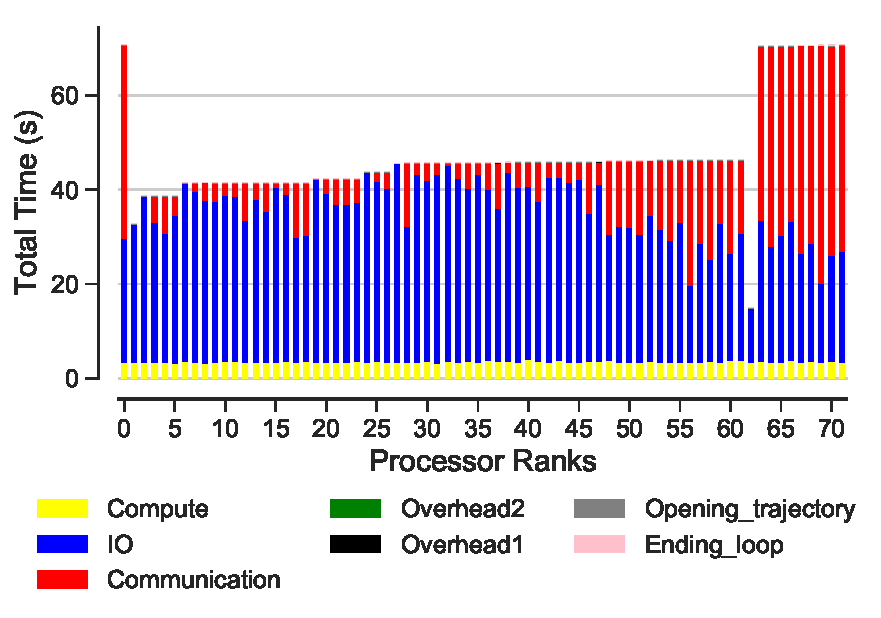
\includegraphics[width=\linewidth]{figures/main-RMSD-BarPlot-rank-comparison_72_4.pdf}
  \caption{Compute \tcomp, IO \tIO, communication \tcomm , ending the for loop $t_{end\_loop}$,
  opening the trajectory $t_{opening\_trajectory}$, and overheads $t_{Overhead1}$,  $t_{Overhead2}$ per MPI rank (as described in methods).}
  \label{fig:MPIranks}
\end{subfigure}
%
\caption{Performance of the RMSD task with MPI which is I/O-bound $\tcomp/\tIO \approx 0.3$.
Data are read from the file system (I/O included) and results are communicated back to
  rank 0 (communications included).}
\label{fig:MPIwithIO}
\end{figure}

\subsubsection*{Identification of Scalability Bottleneck}

Figure \ref{fig:ScalingComputeIO} shows the scaling of \tcomp and \tIO individulally. 
As shown, \tcomp scales very well; however, \tIO does not show good scaling beyond a single node (24 cores) and that explains why we are seeing these variations in \tIO across different ranks (Figure \ref{fig:MPIranks}). 
Considering the results in Figures \ref{fig:MPIwithIO} and \ref{fig:ScalingComputeIO}, we can conclude that communication and I/O are the root causes for stragglers. 

\begin{figure}
\centering
  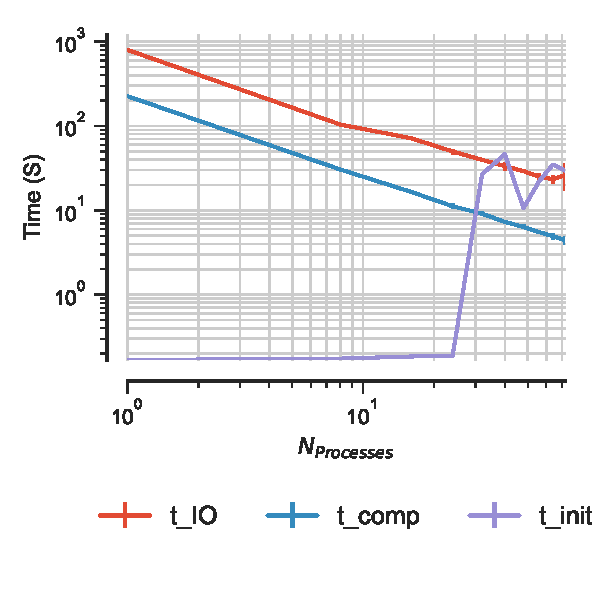
\includegraphics[width=\linewidth]{figures/main-RMSD-time_comp_IO_comparison.pdf}
\caption{Scaling of the \tcomp and \tIO of the RMSD task with MPI.}
\label{fig:ScalingComputeIO}
\end{figure}

\subsubsection*{Hardware}

We did not discern any specific patterns that could be traced to the underlying hardware. Stragglers were observed on \emph{SDSC Comet},
\emph{TACC Stampede} and \emph{TACC Data Analytics System Wrangler} (data not shown). There was also no clear pattern in which certain MPI
ranks would always be a straggler and we could also not trace stragglers to specific cores or nodes (or at least our data did not
reveal an obvious pattern). Therefore, the phenomenon of stragglers in the RMSD test appears to be independent from the underlying hardware.

\subsection{Dihedral Featurization Benchmarks}
\label{DF}
We briefly tested a much larger computational workload ($t_{compute_{per-frame}}$ = 40 ms, $t_{IO_{per-frame}}$ = 0.4 ms, thus $\tcomp/\tIO \approx 100$), namely dihedral
featurization on \emph{Comet} with Infiniband and Lustre file system.

The system scales linearly and close to ideal (Figure \ref{fig:MPI-dihedral-comm}). Although, there is communication of large
result arrays, which is costly for multiple ranks, the speed-up curve (Eq.~\ref{eq:speedup}) in Figure \ref{fig:MPI-dihedral-comm-speedup}
demonstrates very good scaling with the number of cores (up to 72 cores on 3 nodes).  The reason is that the communication cost (for
$MPI.Gather()$-lines 36-44 in \ref{alg:Dihedral}) decreases with increasing the number of cores because the result array size that has to be
communicated also decreases (Figure \ref{fig:comparison-t_comm-dihedral}).  Based on Figure \ref{fig:comparison-t_comm-dihedral}, communication scales fairly well
with the number of processes. This can be attributed to larger array sizes compared to the RMSD task and according to \citet{Dalcin:2011aa}
the overhead of the \package{mpi4py} package decreases as the array size to be communicated increases. The dihedral featurization workload
has larger array size for all processor sizes (per task, a time series of feature vectors of size $N_{b} \times (213 \times 2 \times 2$) when
compared to the RMSD workload (per task a float array of length $N_{b}$) and therefore we are hypothesizing that the higher
performance of \package{mpi4py} for larger array sizes has lead to better overall scaling. 
In addition, for higher computational workloads the competition over accessing the file is less severe as compared to lower computational workloads. 
 
\begin{figure}[tbp]
\centering
\begin{subfigure}{.35\textwidth}
  \centering
  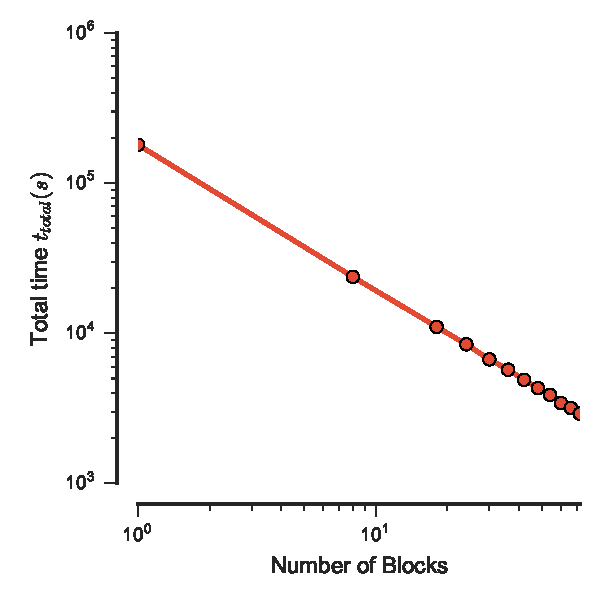
\includegraphics[width=\linewidth]{figs/t_total-dihedral-comm.pdf}
  \caption{Scaling total}
\end{subfigure}
\hfill
\begin{subfigure}{.5\textwidth}
  \centering
  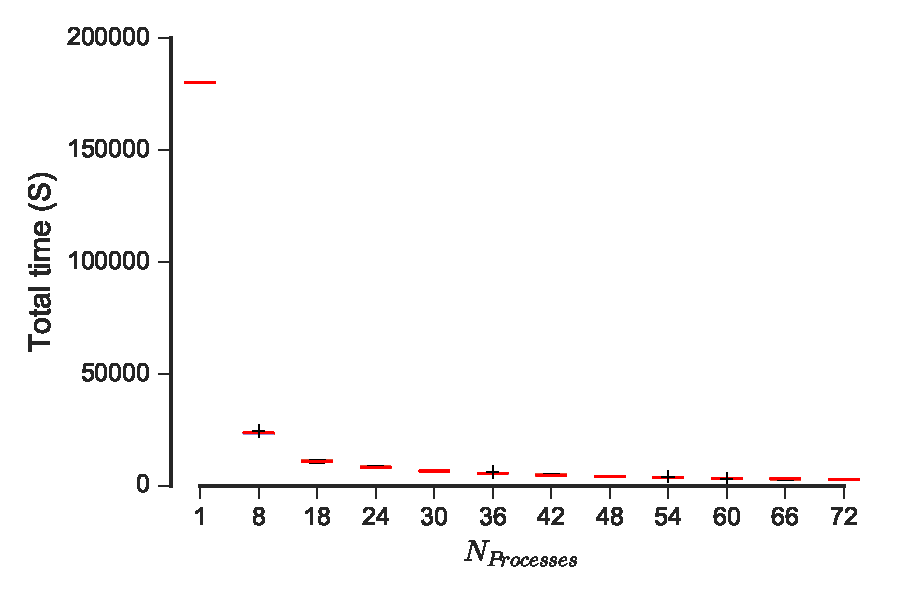
\includegraphics[width=\linewidth]{figs/total_time_boxplot-dihedral-comm.pdf}
  \caption{Total job execution time along with the mean and standard
    deviations across 5 repeats.}
\end{subfigure}
\bigskip

\begin{subfigure} {.35\textwidth}
  \centering
  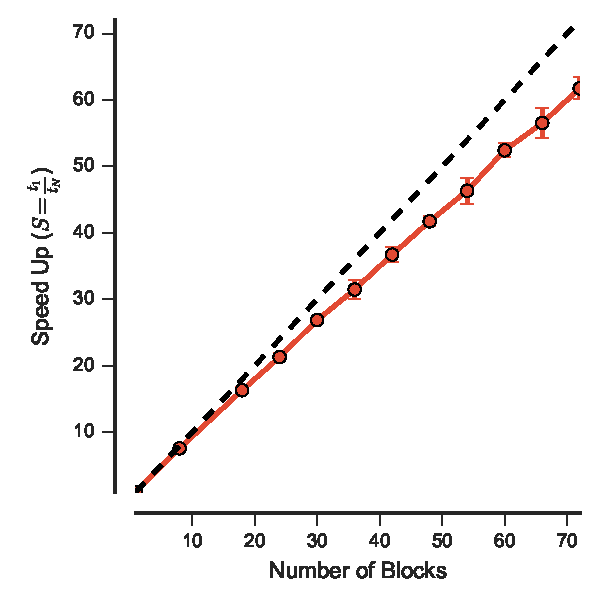
\includegraphics[width=\linewidth]{figs/speed_up-dihedral-comm.pdf}
  \caption{Speed-up}
  \label{fig:MPI-dihedral-comm-speedup}
\end{subfigure}
\hfill
\begin{subfigure} {.5\textwidth}
  \centering
  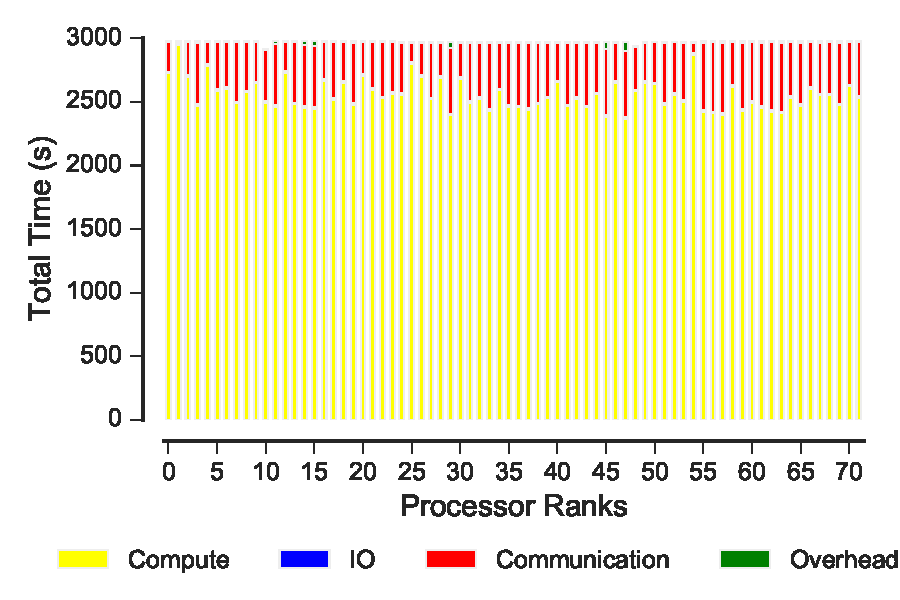
\includegraphics[width=\linewidth]{figs/BarPlot-rank-comparison-dihedral-comm.pdf}
  \caption{time per MPI rank for a typical run (note, IO is almost too
    small to be visible)}
\end{subfigure}
\caption{Performance for the \textbf{dihedral featurization} workload,
  which is compute-bound $\tcomp/\tIO \approx 100$, when
  \emph{communications are included}.}
\label{fig:MPI-dihedral-comm}
\end{figure}

\begin{figure}[tbp]
\centering
\begin{subfigure} {.55\textwidth}
  \centering
  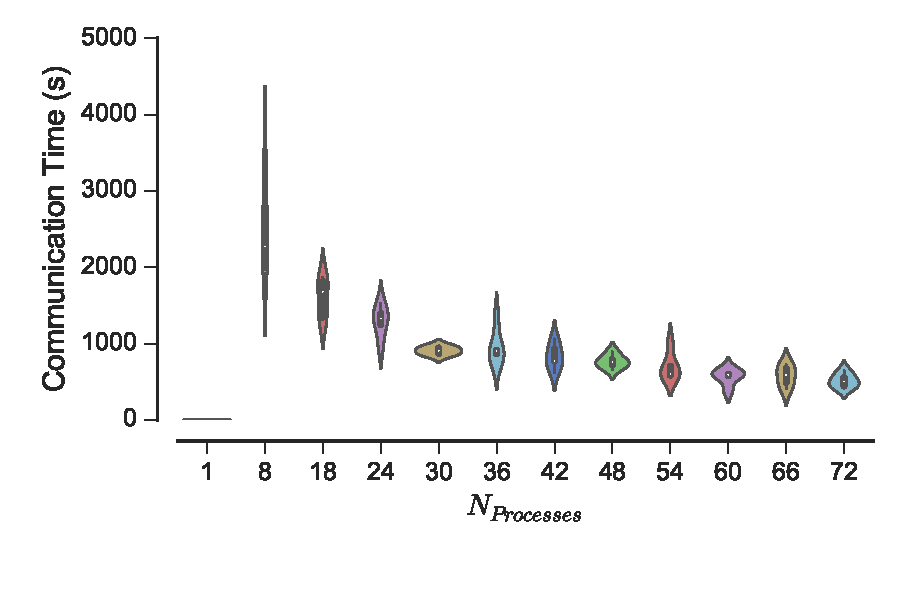
\includegraphics[width=\linewidth]{figs/ViolinPlot-Ncores-comparison-comm-dihedral.pdf}
  \caption{Communication time distribution for different number of
    processes (shown as violin plots \protect\cite{Hintze:1998tw}
    with kernel density estimates as implemented in
    \package{seaborn}); the white dot indicates the median.}
\end{subfigure}
\hfill
\begin{subfigure}{.35\textwidth}
  \centering
  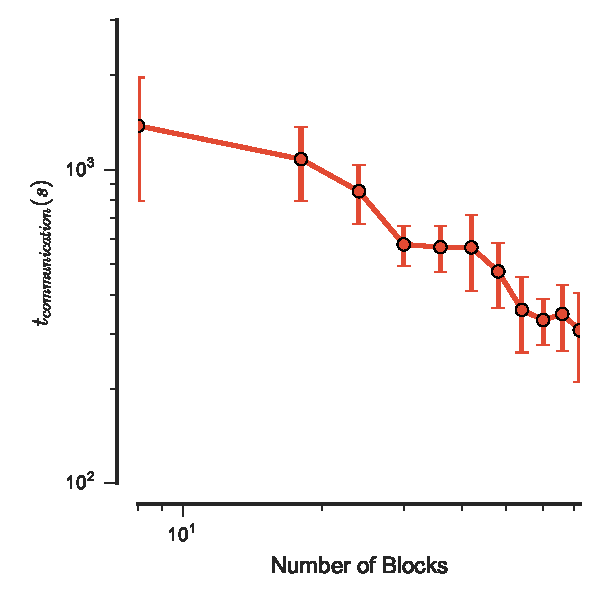
\includegraphics[width=\linewidth]{figs/t_comm-mean-dihedral.pdf}
  \caption{Scaling communcation time (mean and standard deviation)}
\end{subfigure}
\caption{Comparison of communication cost for different number of
  processes over 5 repeats for the \textbf{dihedral featurization}
  workload (with \emph{communications included}).}
\label{fig:comparison-t_comm-dihedral}
\end{figure}

Overall, increasing the computational workload over I/O improves scaling. For large compute-bound workloads such as the dihedral
featurization task, stragglers are eliminated and nearly ideal strong scaling is achieved. 
The fact that linear scaling is possible, even with expensive communications, makes parallelization a valuable strategy to reduce
the total time to solution for large computational workloads. In a real-world application to one of our existing data sets on local
workstations with Gigabit interconnect and Network File System (NFS) (using the Dask parallel library instead of MPI), analysis time was reduced from more
than a week to a few hours (data not shown).

\subsection{Effect of \tcomp/\tIO on Performance}
\label{bound}

The RMSD task turned out to be I/O bound, i.e.,
\begin{gather*}
  \frac{\tcomp}{\tIO} \ll 1.
\end{gather*}

and we were not able to achieve good scaling above a single node. 
However, Dihedral featurization turned out to be compute bound and we were able to achieve near ideal scaling. 
We therefore, hypothesized that decreasing the relative I/O load with respect to compute load would also reduce the stragglers. 
We therefore increased the computational load so that the work became compute bound, i.e.,

\begin{gather*}
  \frac{\tcomp}{\tIO} \gg 1.
\end{gather*}

i.e., now processes are not constantly performing I/O and instead, I/O is interleaved with longer periods of computation.
In order to artificially increase the computational load we repeated the same RMSD calculation (line 10, algorithm \ref{alg:RMSD}) 40, 70 and 100 times in a loop respectively.

\subsubsection{Increased workload (RMSD)}
The RMSD workload was artificially increased forrty-fold, seventy-fold, and hundred-fold and we measured performance as before. 
Figure \ref{fig:tcomp_tIO_effect} shows the effect of $\tcomp/\tIO$ ratio on performance.
On average, each rank took $N_{b} \times \tIO $ (where $N_{b}=N_{\text{frames}}/N$ is the
number of frames per trajectory block, i.e., the number of frames
processed by each MPI rank for $N$ processes) for I/O,
$X \times N_{b} \times \tcomp$ for the $X\times$ RMSD computation.

As the $\tcomp/\tIO$ ratio increases, speed-up and performance improves and 
show overall better scaling than the I/O-bound workload, i.e. $1\times$ RMSD (Figure \ref{fig:S1_tcomp_tIO_effect}).
When $\tcomp/\tIO$ ratio increases, the RMSD calculation consistently scales up to larger numbers of cores ($N=56$ for $70\times$ RMSD).
Figures \ref{fig:S2_tcomp_tIO_effect} and \ref{fig:E_tcomp_tIO_effect} shows the improvment in performance more clearly.
In fact, as the $\tcomp/\tIO$ ratio increases, the values of speed-up and efficiency get closer to their ideal value for each number of processor counts.  

\begin{figure}
\centering
\begin{subfigure} {.3\textwidth}
  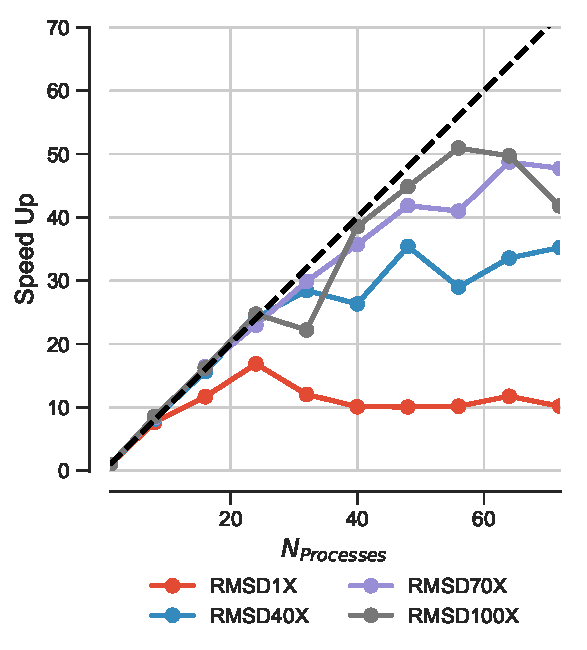
\includegraphics[width=\linewidth]{figures/Compute_to_IO_ratio_on_performance_2d_v17.pdf}
  \caption{Effect of \tcomp/\tIO on the Speed-Up}
  \label{fig:S1_tcomp_tIO_effect}
\end{subfigure}
\hfill
\begin{subfigure}{.3\textwidth}
  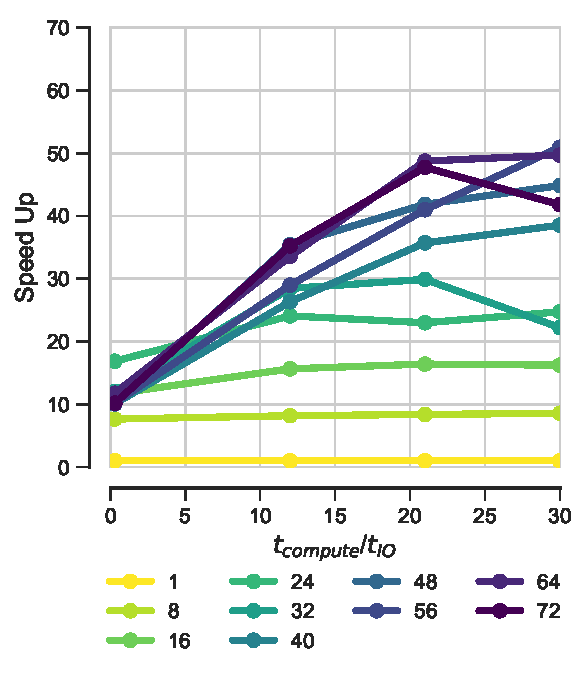
\includegraphics[width=\linewidth]{figures/Compute_to_IO_ratio_on_performance_2d_2_v17.pdf}
  \caption{Change in the Speed-Up with respect to \tcomp/\tIO for different processor counts}
  \label{fig:S2_tcomp_tIO_effect}
\end{subfigure}
\hfill
\begin{subfigure}{.3\textwidth}
  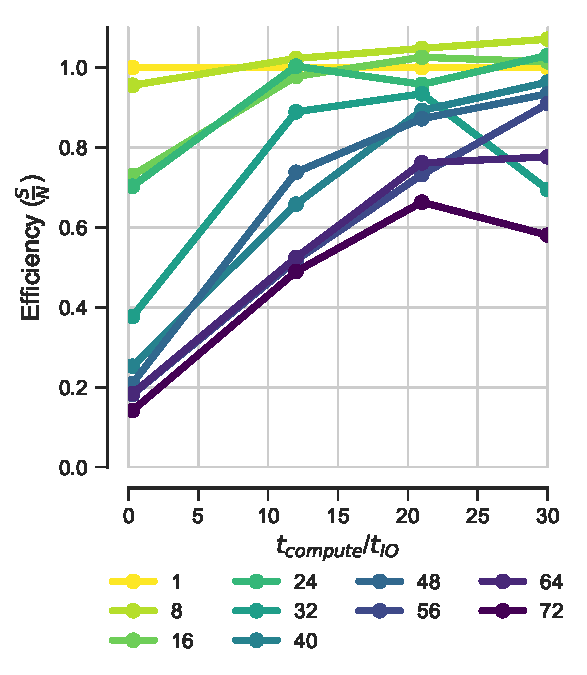
\includegraphics[width=\linewidth]{figures/Compute_to_IO_ratio_on_performance_2d_3_v17.pdf}
  \caption{Change in the efficiency with respect to \tcomp/\tIO for different processor counts}
  \label{fig:E_tcomp_tIO_effect}
\end{subfigure}
%
\caption{Performance change of the RMSD task with MPI with different $\tcomp/\tIO$ ratios. We tested performance for $\tcomp/\tIO$ ratios of 0.3, 12, 21, 30
which correspond to $1\times$ RMSD, $40\times$ RMSD, $70\times$ RMSD, and $100\times$ RMSD respectively (communication is included)}
\label{fig:tcomp_tIO_effect}
\end{figure}

Even for moderately compute-bound workloads such
as the $40\times$ and $70\times$ RMSD tasks, increasing the computational workload over I/O reduced the impact of stragglers even
though they still contribute to large variations in timing across different ranks and thus to somewhat erratic scaling. 

Given the results for Dihedral featurization and RMSD algorithms (Algorithms \ref{alg:Dihedral}, and \ref{alg:RMSD}) and $X\times$ RMSD (Figure \ref{fig:tcomp_tIO_effect})
\textbf{we hypothesize that MPI competes with Lustre on the same network interface, which would explain why communication appears to
  be primarily a problem in the presence of I/O when \tcomp/\tIO is small.}
In fact, decreasing the I/O load relative to the compute load should open up the network for communication. 

\subsection{Communication Cost and Application of Global Array}
\label{Global-Array}
As discussed in the previous sections, \ref{fig:MPIranks}, for small \tcomp/\tIO communication acts as the scalability bottleneck. 
In fact, when the processes communicate result arrays back to the master (rank 0) process, some processes take much longer as compared to other processes. 
Now we want to know what strategies can be used to avoid communication cost. 

Algorithm \ref{alg:GA} describes RMSD algorithm in combination with the global array.
In this algorithm, we use global array instead of message passage paradigm to see if we can reduce communication cost. 
Given the speed up plots (Figure \ref{fig:MPIspeedup-ga4py}) and total time scaling (Figure \ref{fig:MPIscaling-ga4py}) global array improves strong scaling performance.
Although communication time has significantly decreased using global array (compare Figure \ref{fig:MPIranks-ga4py} to Figure \ref{fig:MPIranks}),
the existing variation in the dominant I/O part of the calculation would still prevent ideal scaling (Figure \ref{fig:ScalingComputeIO-ga4py}).
In fact, although communications were performed using global arrays, scaling is still far from ideal as a result of slow processes due to I/O variation.
These slow processes take about 50~s, which are slower than the mean execution time of all ranks, i.e. 17~s. 

\begin{algorithm}[t]\mknote{Giannis Could you please check this algorithm too?}
	\scriptsize
    \caption{Global Array instead of Message-Passing Paradigm}
    \label{alg:GA}
    \hspace*{\algorithmicindent} \textbf{Input:} \emph{mobile}: the desired atom groups to perform RMSD on them \\ 
    \hspace*{\algorithmicindent} \emph{bsize}: Total number of frames assigned to each rank $N_{b}$\\
    \hspace*{\algorithmicindent} \emph{g\_a}: Initialized global array of $($ $bsize*size,2$ $)$  \\
    \hspace*{\algorithmicindent} \emph{buf}: Initialized buffer to store final calculated RMSD results of size $($ $bsize*size,2$ $)$  \\
    \hspace*{\algorithmicindent} \emph{xref0}: mobile group in the initial frame which will be considered as rerference \\
    \hspace*{\algorithmicindent} \emph{start \& stop}: that tell which block of trajectory (frames) is assigned to each rank \\
    \hspace*{\algorithmicindent} \emph{topology \& trajectory}: files to read the data structure from \\
    \hspace*{\algorithmicindent} \textbf{Output:} Calculated RMSD arrays
    \begin{algorithmic}[1]
        \State \texttt{bsize = int(np.ceil(mobile.universe.trajectory.n\_frames / float(size)))}
        \State \texttt{g\_a = ga.create(ga.C\_DBL, [bsize*size,2], "RMSD")}
        \State \texttt{buf = np.zeros([bsize*size,2], dtype=float)}
        \\
        \State \texttt{start4 = time.time()}
	\State \texttt{out = Block\_RMSD(index, topology, trajectory, xref0, start=start, stop=stop, step=1)}
	\State \texttt{start5 = time.time()}
	\\
	\State \texttt{ga.put(g\_a, out[:,:], (start,0), (stop,2))}
	\\
	\State \texttt{start6 = time.time()}
	\If{rank == 0}
   	     \State \texttt{buf = ga.get(g\_a, lo=None, hi=None)}
        \EndIf
         \\
         \State \texttt{start7 = time.time()}        
    \end{algorithmic}
\end{algorithm}

\begin{figure}
\centering
\begin{subfigure}{.4\textwidth}
  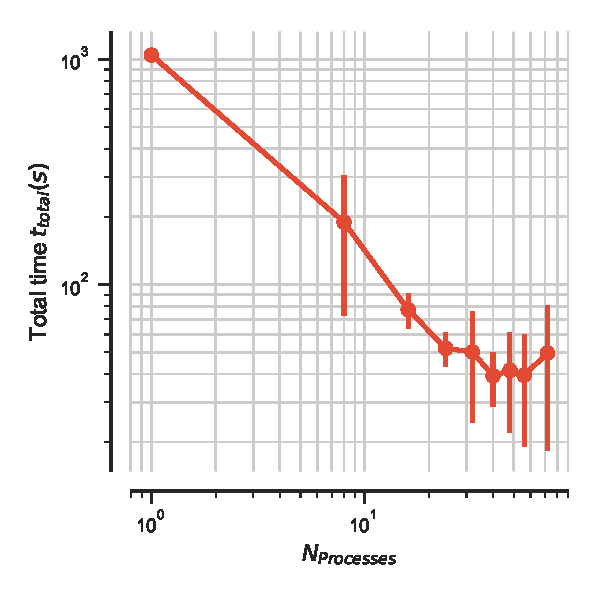
\includegraphics[width=\linewidth]{figures/RMSD-ga4py-t_total.pdf}
  \caption{Scaling total}
  \label{fig:MPIscaling-ga4py}
\end{subfigure}
\hfill
\begin{subfigure}{.4\textwidth}
  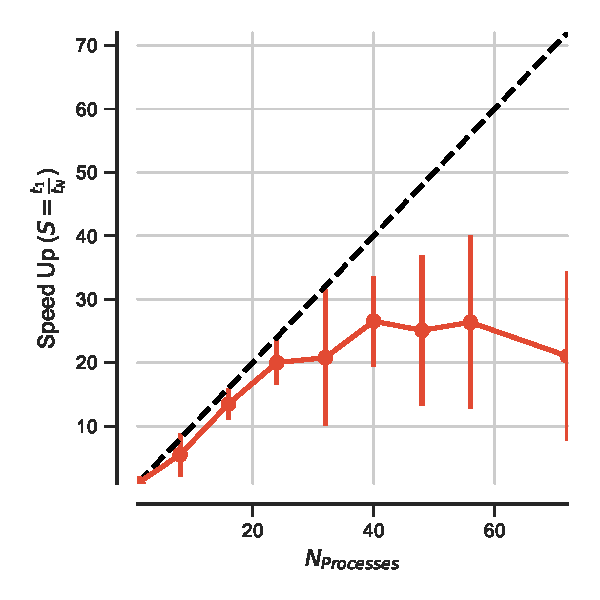
\includegraphics[width=\linewidth]{figures/RMSD-ga4py-speed_up.pdf}
  \caption{Speed-up}
  \label{fig:MPIspeedup-ga4py}
\end{subfigure}
\bigskip

\begin{subfigure} {.8\textwidth}
  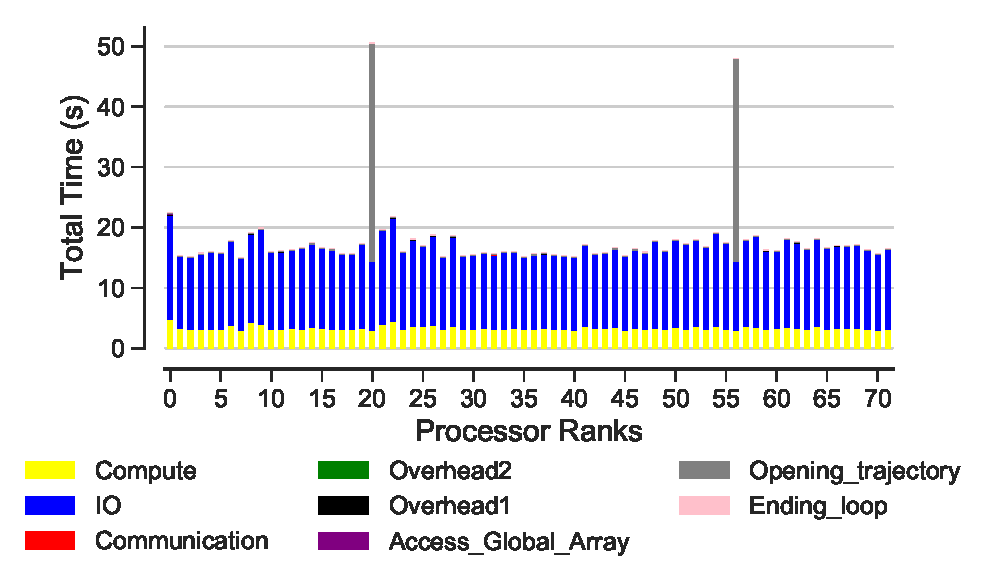
\includegraphics[width=\linewidth]{figures/RMSD-ga4py-BarPlot-rank-comparison_72_1.pdf}
  \caption{Compute \tcomp, IO \tIO, communication \tcomm , ending the for loop $t_{end\_loop}$,
  opening the trajectory $t_{opening\_trajectory}$, and overheads $t_{Overhead1}$,  $t_{Overhead2}$ per MPI rank (as described in methods).}
  \label{fig:MPIranks-ga4py}
\end{subfigure}
%
\caption{Performance of the RMSD task with MPI using global array ($\tcomp/\tIO \approx 0.3$).
Data are read from the file system (I/O included). All ranks update the global array and rank 0 accesses the whole RMSD array through the global memory address.}
\label{fig:MPIwithIO-ga4py}
\end{figure}

\begin{figure}
\centering
  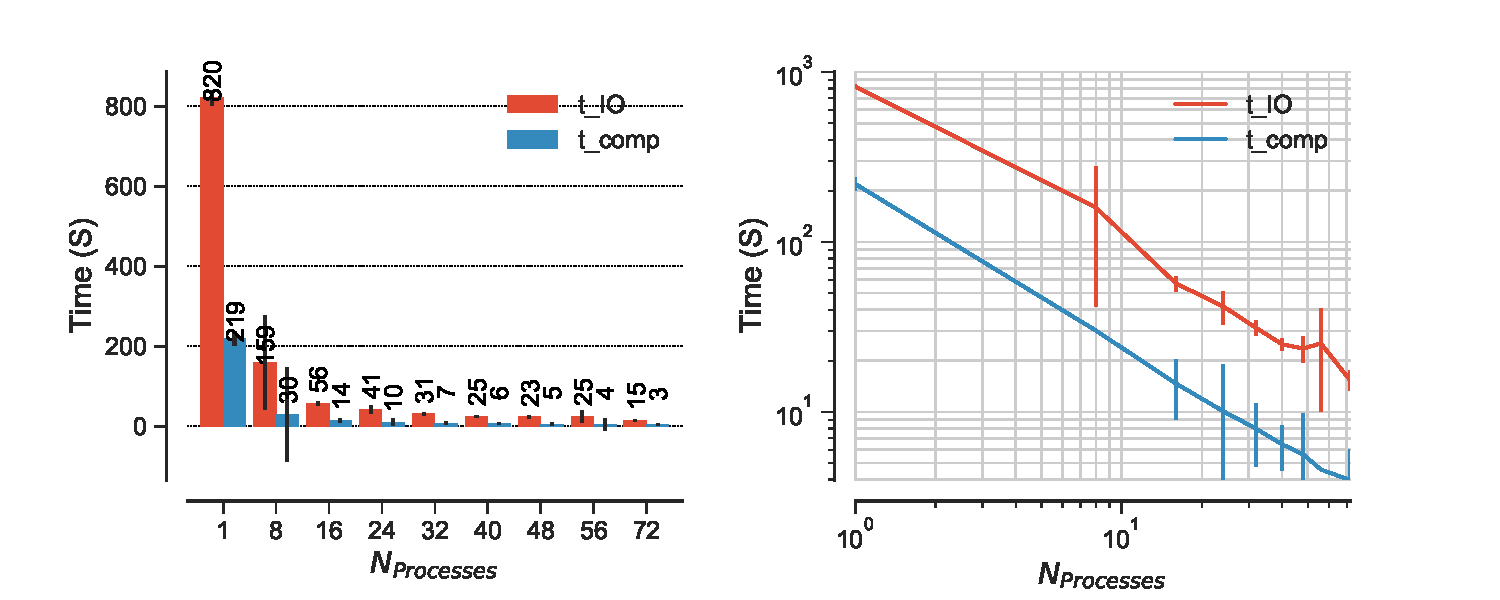
\includegraphics[width=\linewidth]{figures/RMSD-ga4py-time_IO_comparison.pdf}
\caption{Scaling of the \tcomp and \tIO of the RMSD task with Global Array.}
\label{fig:ScalingComputeIO-ga4py}
\end{figure}

\subsection{I/O Cost}
\label{I/O}
We showed previously that the I/O system can have a large effect on the parallel performance of the RMSD task \cite{Khoshlessan:2017ab},
especially because the average time to perform the computation \tcomp (about 0.09 ms) is about three times smaller than the I/O time \tIO (about 0.3 ms) (Figures \ref{fig:ScalingComputeIO} and \ref{fig:MPIwithIO}). 
In fact, poor I/O performance is responsible for the stragglers, and the question is ``are stragglers waiting for file access?". 
Due to the large file size and memory limit, processes are not able to load the whole trajectory into memory at once and as a result each process is only allowed to load one frame into memory at a time.
The test trajectory has about $2,512,200$ frames in total and as a result there will be $2,512,200$ file access requests. 
Thus, when the compute time is small with respect to I/O, then I/O can be a major issue as we also see in our results (Figures \ref{fig:ScalingComputeIO} and \ref{fig:MPIwithIO}).    
Read throughput might be limited by the available bandwidth on the Infini-band network interface that serves the Lustre file system and access to files might be throttled.
In fact, we need to come up with ways and strategies to avoid the competition over file access across different ranks when \tcomp/\tIO ratio is small.
To this aim, we experimented two different ways for reducing I/O cost and examined their effect on the performance.
These two ways include: Splitting the trajectory file into as many segments as number of processes and MPI-based Parallel HDF5.
We discuss these two approaches in detail in the following sections.

\subsubsection{Splitting the Trajectories}
\label{Splitting}
In all the previous benchmarks all processes were using a shared trajectory file.
In order to test our hypothesis that \emph{I/O and communication compete over the network resources with small \tcomp/\tIO ratio}, we splitted our trajectory file into as many trajectory segments as the number of processes.
This means that if we have $N$ processes, the trajectory file is splitted into $N$ segments and each segment will have $N_{b}$ frames in it. 
Through this approach, each process will have access to its own segment and there will be no competition over file accesses. 
For reference, the necessary time for splitting the trajectory file is given in Appendix \ref{sec:splitting-timing}.

\subsubsection*{Performance without Global Array}
We ran a benchmark up to 8 nodes (192 cores) and, we observed rather better scaling behavior with efficiencies above 0.6 (Figure \ref{fig:MPIscaling-split} and \ref{fig:MPIspeedup-split}) and the delay time for stragglers has also reduced from 65 to about 23 (Compare Figure \ref{fig:MPIranks-split} to  \ref{fig:MPIranks}). 
However, the scaling is still far from ideal due to the communication. 
Although the delay due to communication is much smaller as compared to RMSD with a shared trajectory file (Compare Figure \ref{fig:MPIranks-split} to Figure \ref{fig:MPIranks}), it is still delaying several processes and as a result leads to longer job completion time (Figure \ref{fig:MPIranks-split}). 
These delayed tasks impact performance as well and hence the speed-up is not still close to ideal scaling (Figure \ref{fig:MPIspeedup-split}).

\begin{figure}
\centering
\begin{subfigure}{.4\textwidth}
  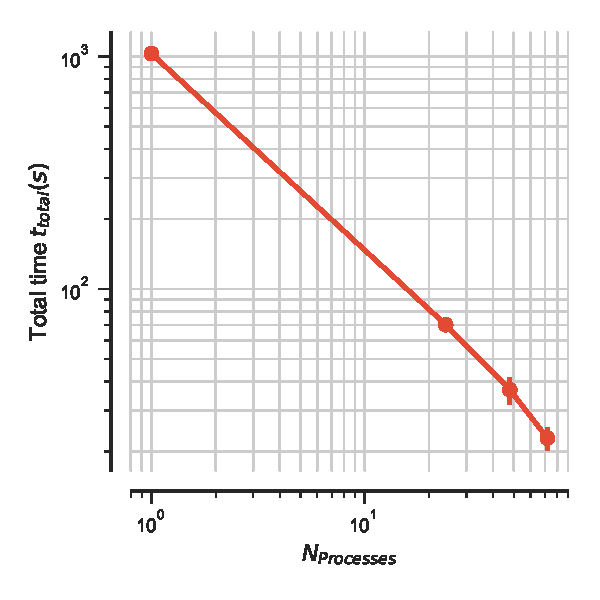
\includegraphics[width=\linewidth]{figures/split-t_total.pdf}
  \caption{Scaling total}
  \label{fig:MPIscaling-split}
\end{subfigure}
\hfill
\begin{subfigure}{.4\textwidth}
  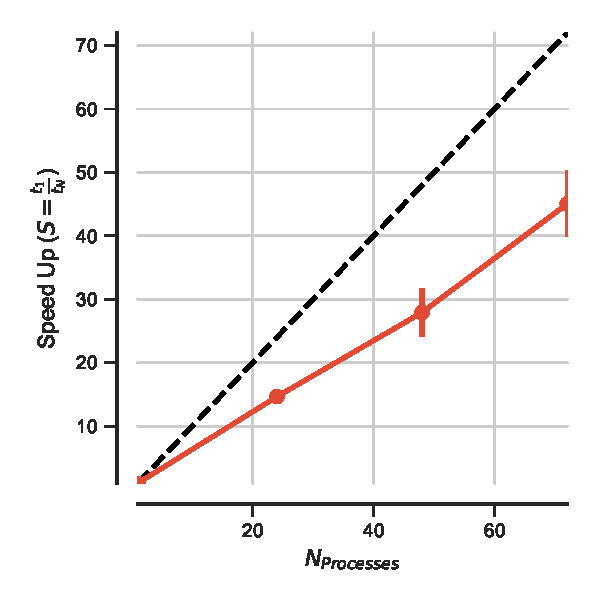
\includegraphics[width=\linewidth]{figures/split-speed_up.pdf}
  \caption{Speed-up}
  \label{fig:MPIspeedup-split}
\end{subfigure}
\bigskip

\begin{subfigure} {.8\textwidth}
  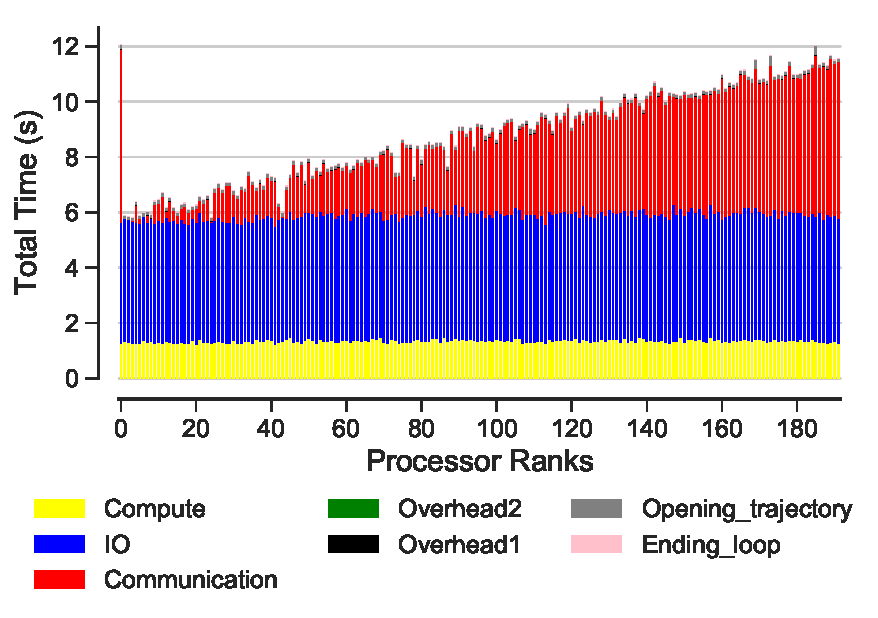
\includegraphics[width=\linewidth]{figures/split-BarPlot-rank-comparison_192_5.pdf}
  \caption{Compute \tcomp, IO \tIO, communication \tcomm , ending the for loop $t_{end\_loop}$,
  opening the trajectory $t_{opening\_trajectory}$, and overheads $t_{Overhead1}$,  $t_{Overhead2}$ per MPI rank (as described in methods).}
  \label{fig:MPIranks-split}
\end{subfigure}
%
\caption{Performance of the RMSD task with MPI using global array ($\tcomp/\tIO \approx 0.3$).
Data are read from the file system (I/O included). All ranks update the global array and rank 0 accesses the whole RMSD array through the global memory address.}
\label{fig:MPIwithIO-split}
\end{figure}

\begin{figure}
\centering
  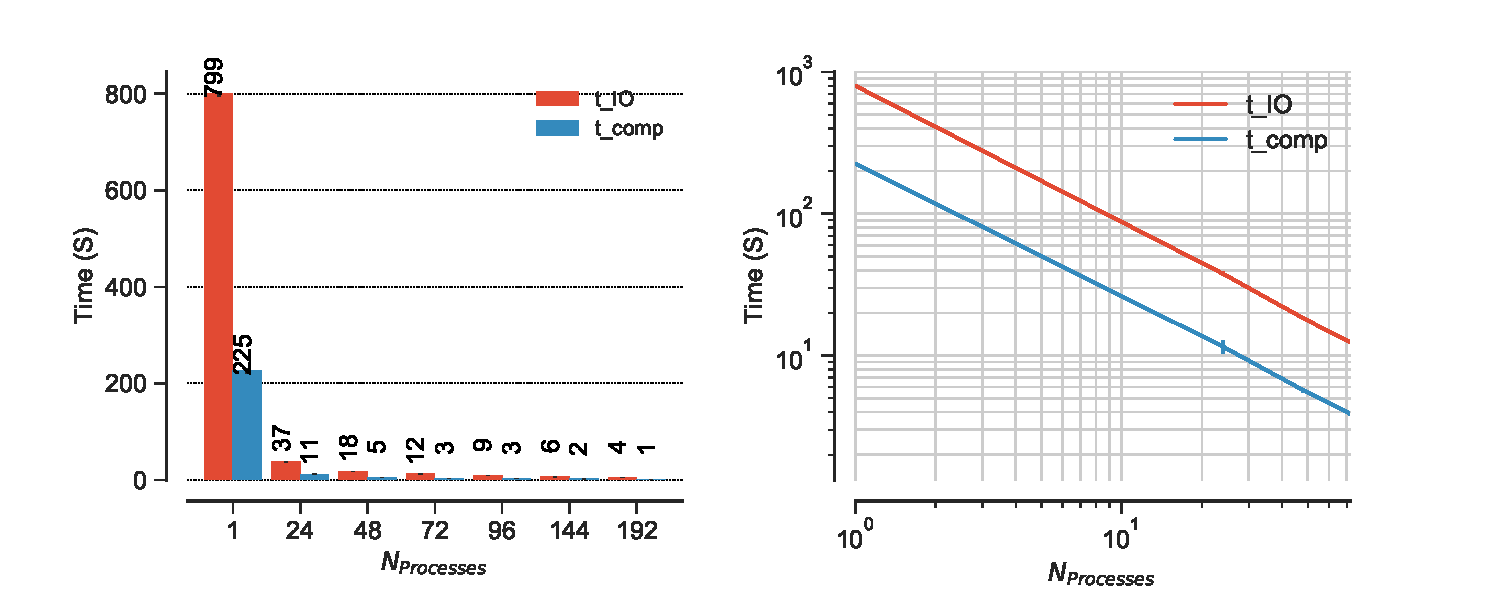
\includegraphics[width=\linewidth]{figures/split-time_comp_IO_comparison.pdf}
\caption{Scaling of the \tcomp and \tIO of the RMSD task with Global Array.}
\label{fig:ScalingComputeIO-split}
\end{figure}

\subsubsection*{Performance using Global Array}
Previously, we showed that global array significantly reduces the communication cost (Section \ref{Global-Array}). 
We want to see how the performance looks like if we split our trajectory file and take advantage of global array.
Again, we ran our benchmark up to 8 nodes (192 cores) and, we observed near ideal scaling behavior with efficiencies above 0.9 (Figure \ref{fig:MPIscaling-split-ga} and \ref{fig:MPIspeedup-split-ga}) with no straggler tasks (Figure \ref{fig:MPIranks-split-ga}).  
The present results show that contention for a file impacts the performance. 
The initial results with splitting the trajectory file suggests that there is in fact an effect, which possibly also interfers with the communications when $\tcomp/\tIO \ll 1$ (i.e. with a I/O bound workload).

\begin{figure}
\centering
\begin{subfigure}{.4\textwidth}
  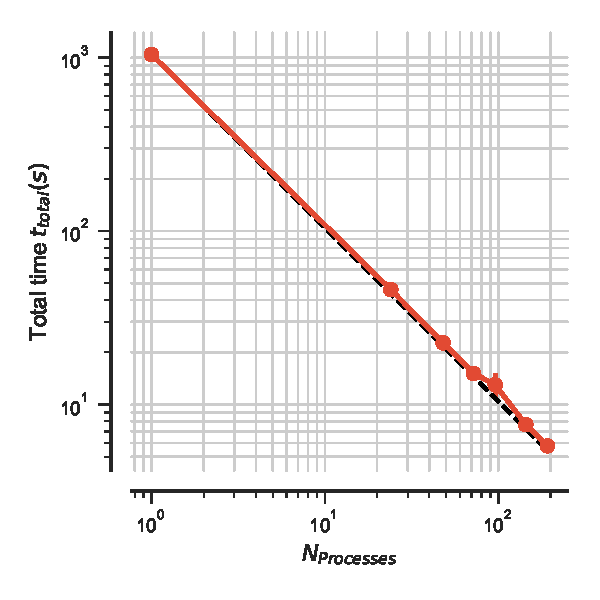
\includegraphics[width=\linewidth]{figures/split-ga-t_total.pdf}
  \caption{Scaling total}
  \label{fig:MPIscaling-split-ga}
\end{subfigure}
\hfill
\begin{subfigure}{.4\textwidth}
  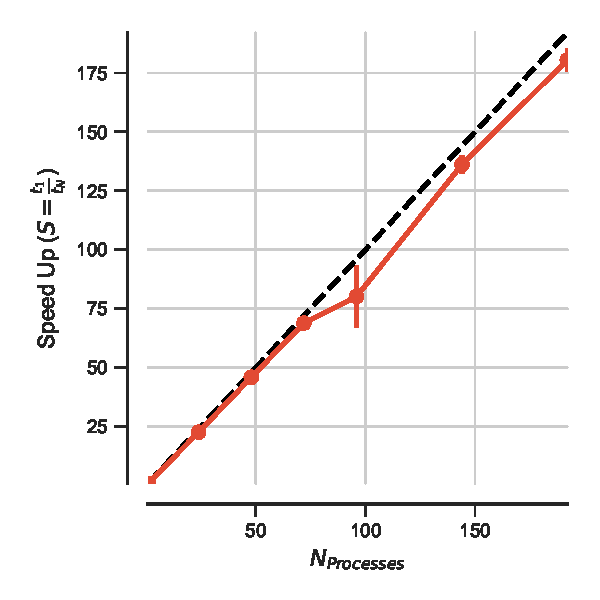
\includegraphics[width=\linewidth]{figures/split-ga-speed_up.pdf}
  \caption{Speed-up}
  \label{fig:MPIspeedup-split-ga}
\end{subfigure}
\bigskip

\begin{subfigure} {.8\textwidth}
  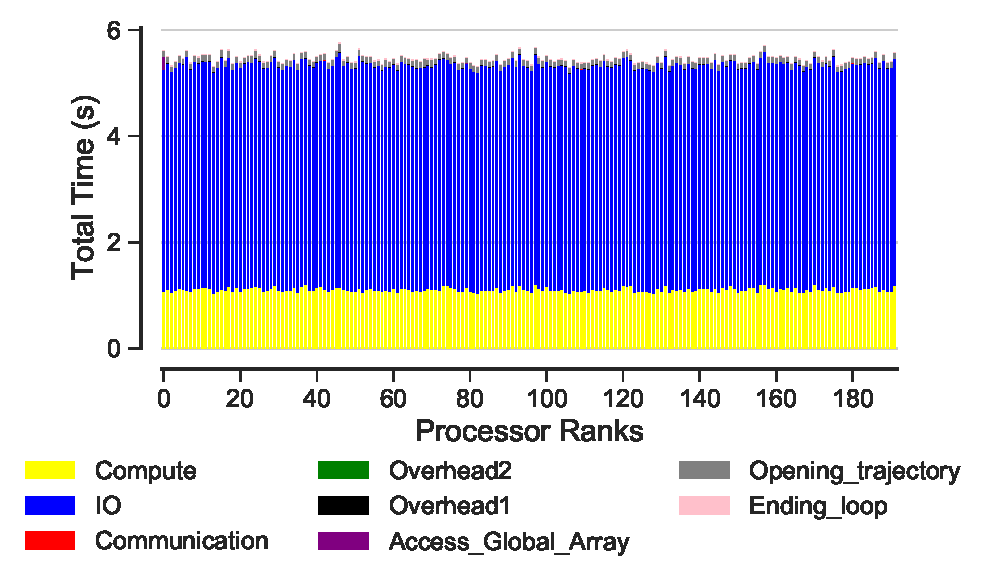
\includegraphics[width=\linewidth]{figures/split-ga-BarPlot-rank-comparison_192_5.pdf}
  \caption{Compute \tcomp, IO \tIO, communication \tcomm , ending the for loop $t_{end\_loop}$,
  opening the trajectory $t_{opening\_trajectory}$, and overheads $t_{Overhead1}$,  $t_{Overhead2}$ per MPI rank (as described in methods).}
  \label{fig:MPIranks-split-ga}
\end{subfigure}
%
\caption{Performance of the RMSD task with MPI using global array ($\tcomp/\tIO \approx 0.3$).
Data are read from the file system (I/O included). All ranks update the global array and rank 0 accesses the whole RMSD array through the global memory address.}
\label{fig:MPIwithIO-split-ga}
\end{figure}

\begin{figure}
\centering
  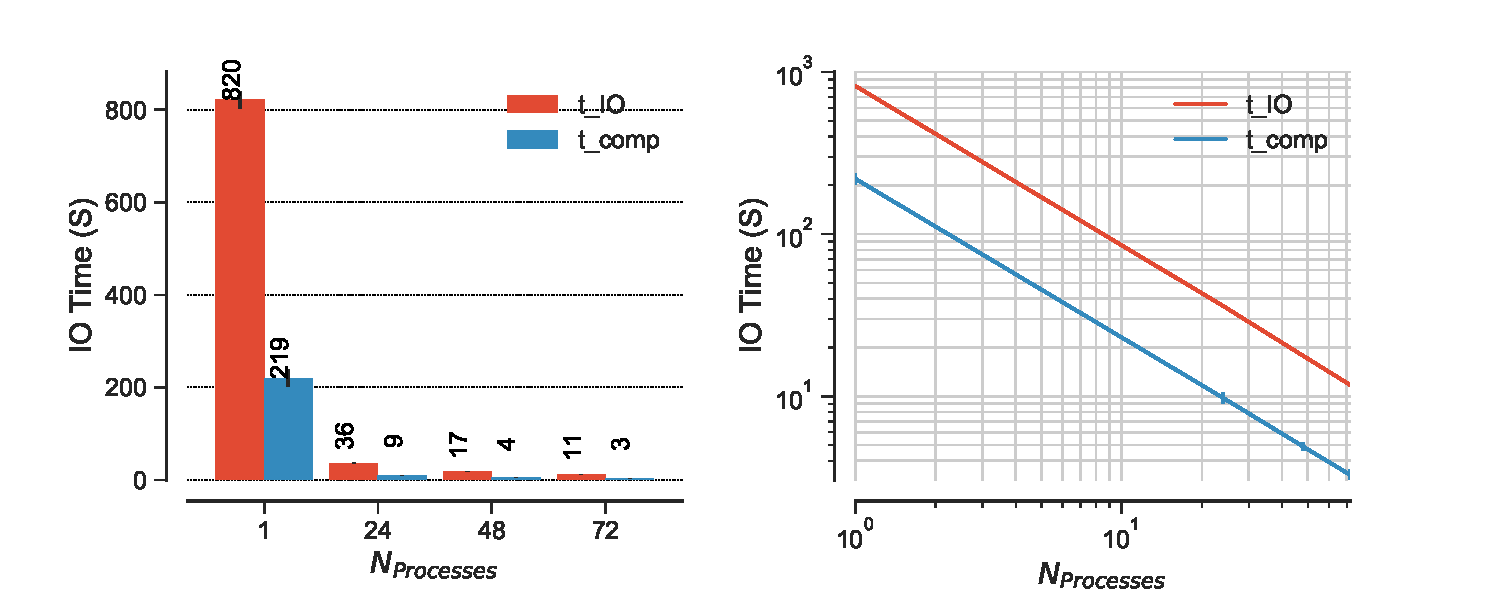
\includegraphics[width=\linewidth]{figures/split-ga-time_IO_comparison.pdf}
\caption{Scaling of the \tcomp and \tIO of the RMSD task with Global Array.}
\label{fig:ScalingComputeIO-split-ga}
\end{figure}

\subsubsection{MPI-based Parallel HDF5}
\label{HDF5}
Another approach we examined to improve I/O scaling is MPI-based Parallel HDF5. 
We converted our XTC trajectory file into HDF5 format so that we can test the performance of parallel IO with HDF5 file format.
The time it took to convert our XTC file with $2,512,200$ frames into HDF5 format was about $5400~s$ in our local resources with network file system (NFS).
Again, we ran our benchmark up to 8 nodes (192 cores) and, we observed near ideal scaling behavior with efficiencies above 0.8 (Figure \ref{fig:MPIscaling-hdf5} and \ref{fig:MPIspeedup-hdf5}) with no straggler tasks (Figure \ref{fig:MPIranks-hdf5}).  
When we split our trajectory, scaling is better as compared to that of parallel I/O (Compare Figure \ref{fig:MPIspeedup-hdf5} to Figure \ref{fig:MPIspeedup-split-ga}). 
However, both methods scale very well up to 8 nodes and have comparable performance.  

\begin{figure}
\centering
\begin{subfigure}{.4\textwidth}
  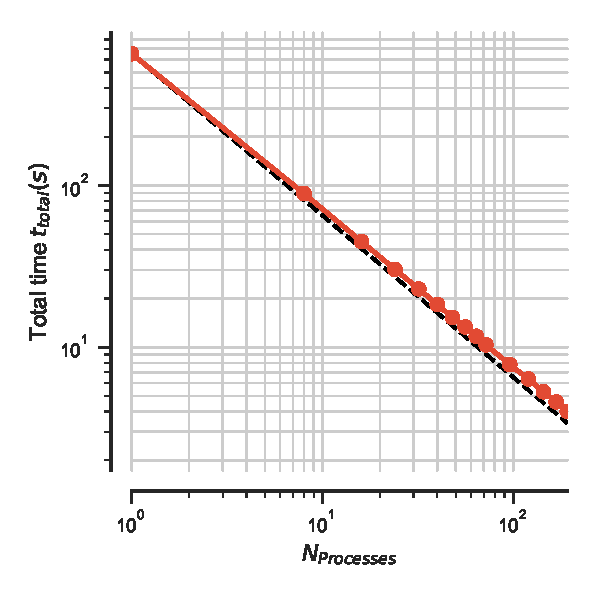
\includegraphics[width=\linewidth]{figures/hdf5-t_total.pdf}
  \caption{Scaling total}
  \label{fig:MPIscaling-hdf5}
\end{subfigure}
\hfill
\begin{subfigure}{.4\textwidth}
  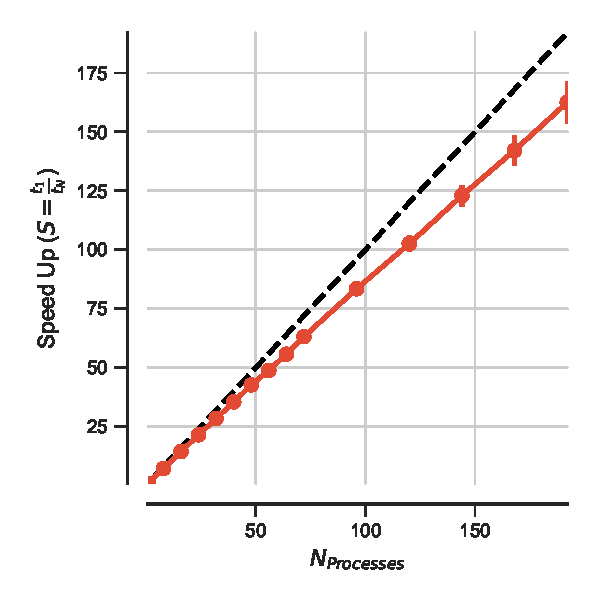
\includegraphics[width=\linewidth]{figures/hdf5-speed_up.pdf}
  \caption{Speed-up}
  \label{fig:MPIspeedup-hdf5}
\end{subfigure}
\bigskip

\begin{subfigure} {.8\textwidth}
  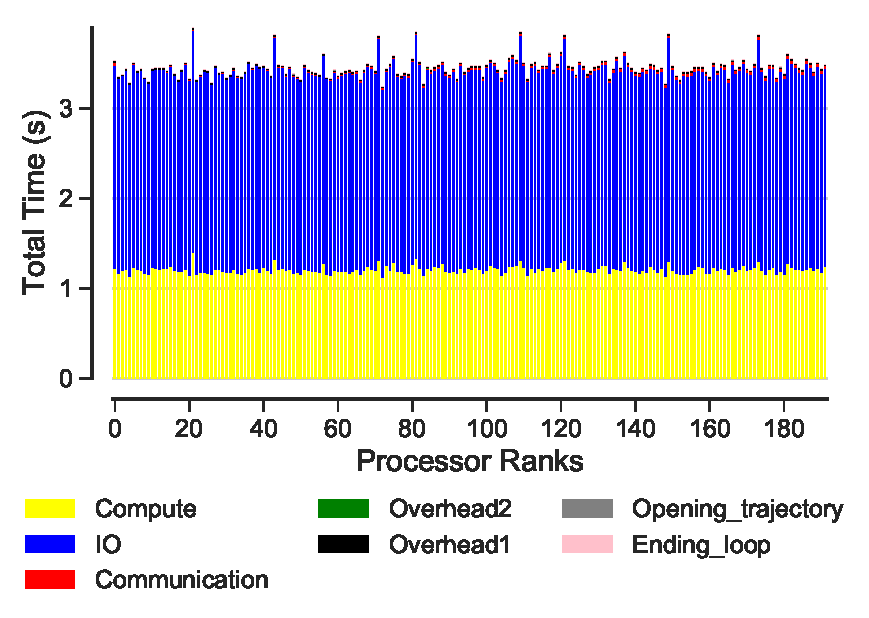
\includegraphics[width=\linewidth]{figures/hdf5-BarPlot-rank-comparison_192_4.pdf}
  \caption{Compute \tcomp, IO \tIO, communication \tcomm , ending the for loop $t_{end\_loop}$,
  opening the trajectory $t_{opening\_trajectory}$, and overheads $t_{Overhead1}$,  $t_{Overhead2}$ per MPI rank (as described in methods).}
  \label{fig:MPIranks-hdf5}
\end{subfigure}
%
\caption{Performance of the RMSD task with MPI-based parallel HDF5 ($\tcomp/\tIO \approx 0.3$).
Data are read from the file system from a shared HDF5 file instead of XTC format (Independent I/O).}
\label{fig:MPIwithIO-hdf5}
\end{figure}

\begin{figure}
\centering
  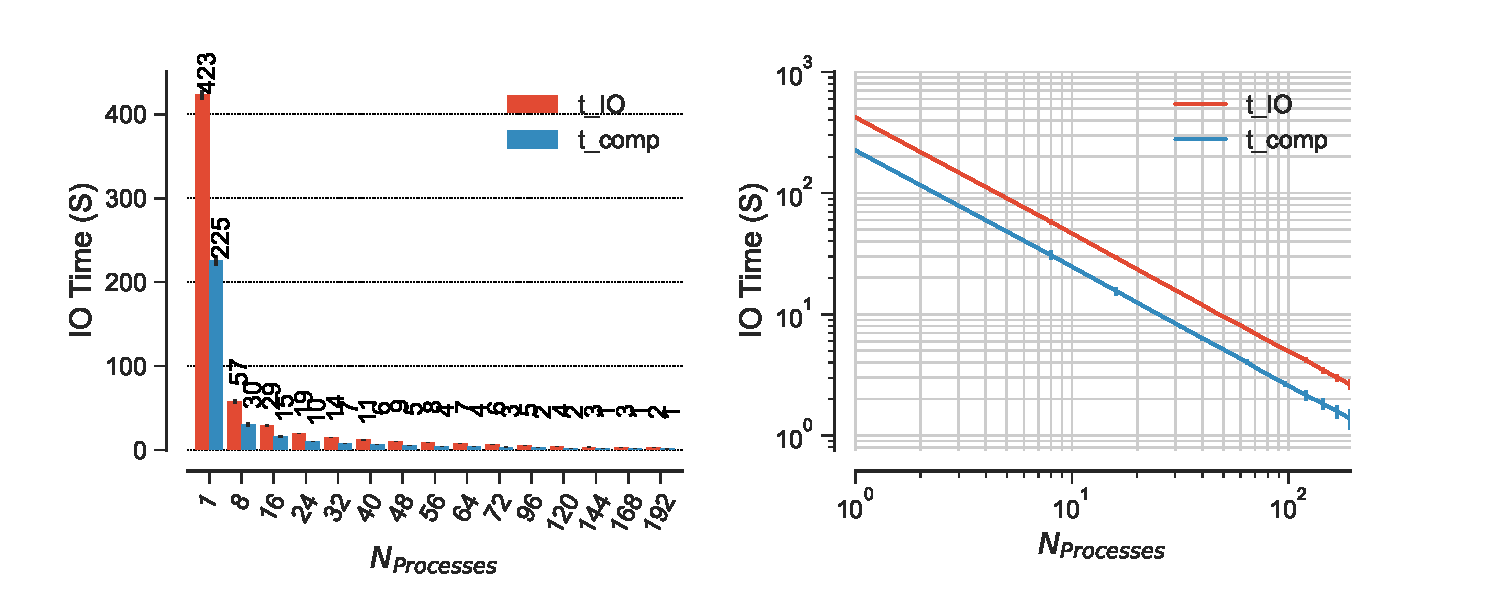
\includegraphics[width=\linewidth]{figures/hdf5-time_IO_comparison.pdf}
\caption{Scaling of the \tcomp and \tIO of the RMSD task with MPI-based parallel HDF5 (Independent I/O).}
\label{fig:ScalingComputeIO-hdf5}
\end{figure}


